\chapter{RESULTS AND DISCUSSION}
\label{chap:resultsandiscussion}

% Ubah bagian-bagian berikut dengan isi dari pengujian dan analisis

This section discusses and shows the results from our test and analysis on training humanoid robot model, human model comparison, and also compares their suitability.
All tests were conducted using the Ichiro robot in the \emph{Robot Cerdas} Laboratory with computer specifications as can be seen in Table \ref{tb:computerspecichiro}.

\def\arraystretch{1.5}
\begin{longtable}{|c|c|}
  \caption{Computer specification on Ichiro robot.}
  \label{tb:computerspecichiro}\\
  \hline
  OS      & Ubuntu 20.04.2 LTS \\
  \hline
  CPU     & Intel i5-10210U (8) @ 4.200GHz \\
  \hline
  GPU     & Intel UHD Graphics  \\
  \hline
  RAM     & 3636 MiB \\
  \hline
\end{longtable}


\section{New Dataset Statistics}
\label{sec:new-dataset-statistics}

This new dataset is a merge of the HumanoidRobotPose dataset and Ichiro's pose dataset. Figure \ref{fig:nimbro-statistics} shows the statistics for the HumanoidRobotPose dataset and Figure \ref{fig:new-dataset-statistics} shows the statistics for the new dataset.
\begin{figure}[ht]
  \centering
  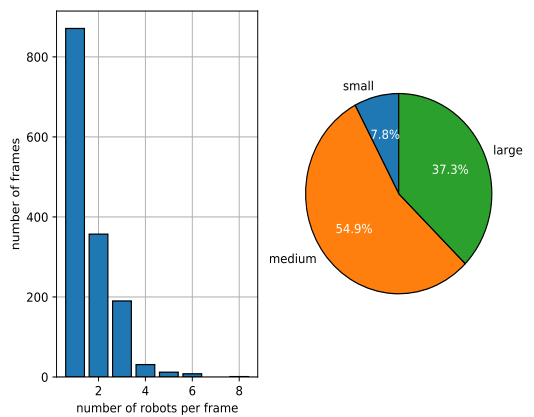
\includegraphics[scale=0.8]{gambar/old_dataset.png}
  \caption{HumanoidRobotPose Statistics.}
  \label{fig:nimbro-statistics}
\end{figure}
The diversity of the number of robot instances per image is illustrated on the left, and the scale proportions of robot instances is shown on the right. The definition of small, medium, and large scale is identical to the COCO dataset.
Most of the additions (Ichiro's pose dataset) are one robot instance (from approximately 850 to 1700) and few are two instances per image (from approximately 380 to 430) with large scale, i.e., (segment area \textgreater 96\textsuperscript{2}). 
This was based on a system requirement that only need pose estimation for one robot and since the distance between the camera and the robot is not that far, the robot object in the image is mainly on a large scale.
\begin{figure}[ht]
  \centering
  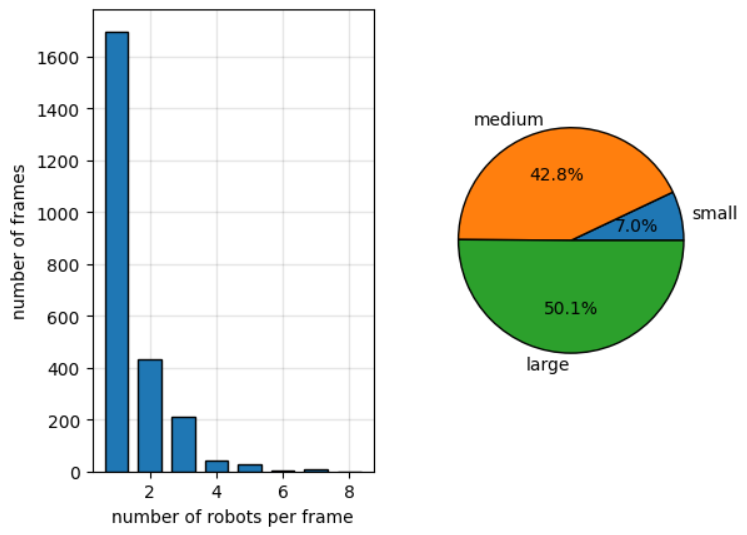
\includegraphics[scale=0.63]{gambar/new_dataset.png}
  \caption{New Dataset Statistics.}
  \label{fig:new-dataset-statistics}
\end{figure}


\section{Robot's Model Training Result}
\label{sec:robotmodeltrainingresult}

This section shows training graphics, evaluation metrics about three models, and testing we perform such as visualizing detection results and inference time.
Figure \ref{fig:nimbro-training-graphics} and \ref{fig:rcnn-training-graphics} show graphics for training loss (on the left) and validation loss (on the right).
Training loss and validation loss of NimbRo's model decreased from 0.02 to 0.0006 and 0.0065 to 0.002 respectively. From Figure \ref{fig:rcnn-training-graphics},
we also can know that training loss and validation loss of Keypoint RCNN decreased from 6 to 2 and 5 to 4 respectively and they were stagnant until the end of the training process.
\begin{figure}[ht]
  \centering
  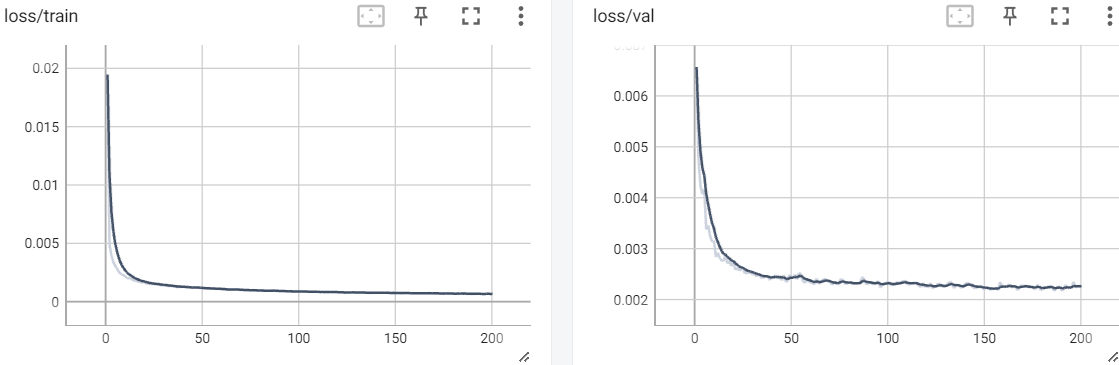
\includegraphics[scale=0.65]{gambar/loss-nimbro.png}
  \caption{Nimbro Training Graphics.}
  \label{fig:nimbro-training-graphics}
\end{figure}
\begin{figure}[ht]
  \centering
  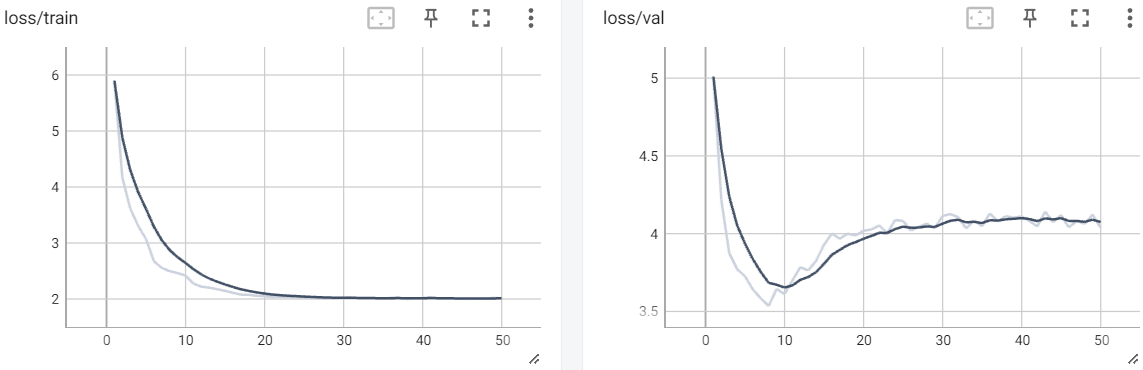
\includegraphics[scale=0.65]{gambar/loss-rcnn.png}
  \caption{Keypoint RCNN Training Graphics.}
  \label{fig:rcnn-training-graphics}
\end{figure}

For the evaluation metrics, NimbRo's Model and Keypoint RCNN use the Object Keypoint Similarity (OKS) with a per-keypoint constant equal to 0.4 for all keypoints.
YOLO also uses OKS, they follow COCO pose estimation standard evaluation metric.
In keypoint detection tasks, precision and recall are commonly used as primary metrics because it measures the quality of predictions (precision measures the proportion of correctly predicted keypoints out of all the keypoints prediction and
  recall measures the proportion of correctly predicted keypoints out of all the actual ground truth). Meanwhile, accuracy is not a relevant metric in keypoint detection because it does not capture the nature of the task effectively.
The task is focused on localizing and identifying keypoints in an image, rather than classifying the entire image or predicting discrete categories. Thus, measuring accuracy, which typically evaluates overall correctness in classification tasks,
  may not provide meaningful insights for this task. Moreover, if we want to get accuracy, we need to know the value of True Negative (TN). Since keypoint detection is not a binary classification task (like classifying the absence or presence of keypoints),
  determining the True Negatives can be challenging. Therefore, the concept of True Negatives is not directly applicable or relevant in this context.

The results on the test set are reported in Table \ref{tb:result-on-test-set}. It can be seen that Keypoint RCNN outperforms other methods in all metrics except for medium scale.
Moreover, Keypoint RCNN showed the best detection results as shown in Table \ref{tb:robotmodelcomparisondetectionresults}, followed by NimbRo's Model and YOLO-pose.
Lastly, NimbRo's Model is the most likely to be applied to real-time systems because it has the lowest inference time as shown in Table \ref{tb:inferencerobot}.
However, since the in PLAY mode, we can do the pose estimation for both human and humanoid robot in the end, not in real-time.
We decide to store the images first and do pose comparisons afterward. Since we are more concerned with a reliable model than a faster model so the Keypoint RCNN model is suitable for this study.

\begin{longtable}{|L{1.5cm}|c|c|c|c|c|c|c|c|c|c|}
  \caption{Results on the test set.}
  \label{tb:result-on-test-set}\\
  \hline
  \rowcolor[HTML]{C0C0C0}
  \textbf{Model} & \textbf{AP} & \textbf{AP\textsubscript{50}} & \textbf{AP\textsubscript{75}} & \textbf{AP\textsubscript{M}} & \textbf{AP\textsubscript{L}} & \textbf{AR} & \textbf{AR\textsubscript{50}} & \textbf{AR\textsubscript{75}} & \textbf{AR\textsubscript{M}} & \textbf{AR\textsubscript{L}} \\
  \hline
  NimbRo Model & 0.828       & 0.879                         & 0.840                         & \textbf{0.886}                       & 0.864                        & 0.836       & 0.884                         & 0.849                         & 0.895                        & 0.872 \\
  \hline                        
  Keypoint RCNN  & \textbf{0.879}       & \textbf{0.936}                         & \textbf{0.904}                         & 0.859                        & \textbf{0.937}                       & \textbf{0.925}       & \textbf{0.973}                         & \textbf{0.944}                         & \textbf{0.936}                        & \textbf{0.955} \\
  \hline                        
  YOLO-pose      & 0.849       & 0.838                         & -                             & -                            & -                            & 0.814       & -                             & -                             & -                            & - \\
  \hline
\end{longtable}

\def\arraystretch{0.5}
\begin{longtable}{|c|c|c|}
  \caption{Robot Model Comparison Detection Results.}
  \label{tb:robotmodelcomparisondetectionresults}\\
  \hline
  \rowcolor[HTML]{C0C0C0}
  \textbf{NimbRo's Model}    & \textbf{Keypoint RCNN} & \textbf{YOLO-pose}\\
  \hline
  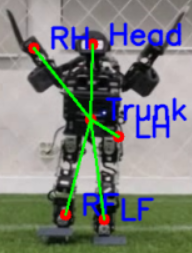
\includegraphics[scale=0.85]{gambar/nimbro-1.png} & 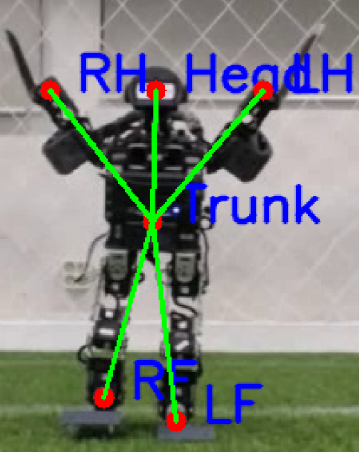
\includegraphics[scale=0.48]{gambar/rcnn-1.png} & 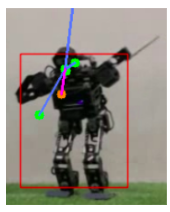
\includegraphics[scale=0.66]{gambar/yolo-1.png} \\
  \hline
  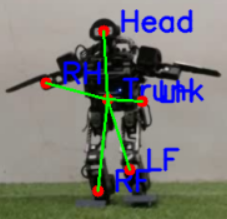
\includegraphics[scale=0.85]{gambar/nimbro-2.png} & 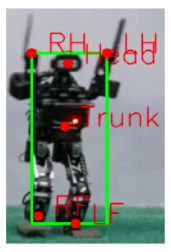
\includegraphics[scale=0.49]{gambar/rcnn-2.png} & 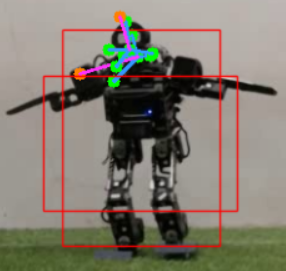
\includegraphics[scale=0.68]{gambar/yolo-2.png} \\
  \hline
  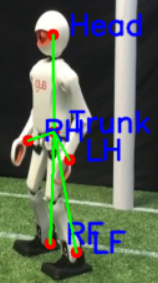
\includegraphics[scale=0.85]{gambar/nimbro-3.png} & 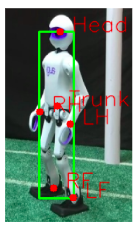
\includegraphics[scale=0.49]{gambar/rcnn-3.png} & 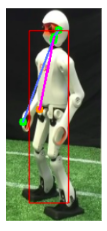
\includegraphics[scale=0.67]{gambar/yolo-3.png} \\
  \hline
\end{longtable}

\def\arraystretch{1.5}
\begin{longtable}{|c|c|c|}
  \caption{Inference Time Model Humanoid Robot.}
  \label{tb:inferencerobot}\\
  \hline
  \rowcolor[HTML]{C0C0C0}
  \textbf{Model}    & \textbf{PyTorch (s)} & \textbf{OpenVINO (s)}\\
  \hline
  NimbRo's Model & 0.4 - 0.5 & 0.15 - 0.2 \\
  \hline
  Keypoint RCNN  & 3.5 - 4.0 & 1.25 \\
  \hline
  YOLO-pose      & 0.7 - 0.75& 0.27 - 0.3 \\
  \hline
\end{longtable}


\section{Human's Model Comparison}
\label{sec:humanmodelcomparison}

Based on \parencite{bazarevsky2020} that compares three different models: BlazePose Lite, BlazePose Full, and OpenPose (body only), they test the models on AR Dataset and Yoga Dataset. As an evaluation metric, they use the Percent of Correct Points with 20\% tolerance (PCK@0.2)
(where assuming the point to be detected correctly if the 2D Euclidian error is smaller than 20\% of the corresponding person's torso size). BlazePose shows slightly worse performance than the OpenPose model on the AR dataset but BlazePose Full outperforms OpenPose on Yoga/Fitness use cases.
Note that, in this study, we use BlazePose Full because by default the value of \emph{model complexity} argument is 1 in the \emph{mediapipe.solutions.pose.Pose} API class. Mediapipe provides 3 BlazePose models: BlazePose Lite, BlazePose Full, and BlazePose Heavy. Pose landmark accuracy as well as inference latency generally go up with the model complexity.
Table \ref{tb:yoloandmediapipecomparison} shows the comparison between YOLO-pose and MediaPipe Pose and based on our needs to just detect one person, MediaPipe should be the best and also reliable choice.  

\begin{longtable}{|L{3cm}|L{5cm}|L{5cm}|}
  \caption{YOLO-pose and MediaPipe Pose Comparison.}
  \label{tb:yoloandmediapipecomparison}\\
  \hline
  \rowcolor[HTML]{C0C0C0}
  \textbf{Features}    & \textbf{YOLO-pose} & \textbf{MediaPipe Pose}\\
  \hline
  Topology             & 17 Keypoints COCO  & 33 Keypoints COCO \\
  \hline
  Workflow             & Detection runs for all frames & Detection runs once followed by tracker until occlusion occurs \\
  \hline
  GPU support          & Support for both CPU and GPU & Only CPU \\
  \hline
  Number of persons    & Multi-person & Single person \\
  \hline
\end{longtable}

\begin{longtable}{|c|c|c|}
  \caption{Inference Time Model Human.}
  \label{tb:inferencehuman}\\
  \hline
  \rowcolor[HTML]{C0C0C0}
  \textbf{Model}    & \textbf{Inference Time (s)} \\
  \hline
  Mediapipe   & 0.15 - 0.2\\
  \hline
  OpenPose    & 0.2\\
  \hline
  YOLO-Pose   & 0.7 - 0.75\\
  \hline
\end{longtable}

\section{Comparing the Suitability Between Humanoid Robot Pose and Human Pose Results}
\label{sec:comparingsuitabilityresults}

By using the method in Section \ref{sec:comparing-keypoints}, we get the result from comparing the human pose and robot pose in percentage terms.
We can see the two figures below, in Figure \ref{fig:comparingb} humans make movement that are more like robot than in Figure \ref{fig:comparinga}.
Therefore, the comparison result of Figure \ref{fig:comparingb} is higher at 91\% than Figure \ref{fig:comparinga} with just 79\%.
This indicates that the system can provide an accurate assessment between the poses of humans and robots.
Furthermore, Figure \ref{fig:comparisongtandresult} shows the comparison between ground truth and detection results using Keypoint RCNN for every robot inside the new dataset
(the left side is ground truth and the right side is detection results).

\begin{figure}
  \centering
  \begin{subfigure}[b]{0.45\textwidth}
      \centering
      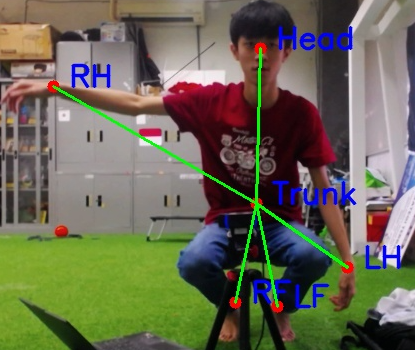
\includegraphics[width=\textwidth]{gambar/human_10_result.jpg}
      \caption{Human Image}
      \label{fig:humanimagea}
  \end{subfigure}
  \hfill
  \begin{subfigure}[b]{0.45\textwidth}
      \centering
      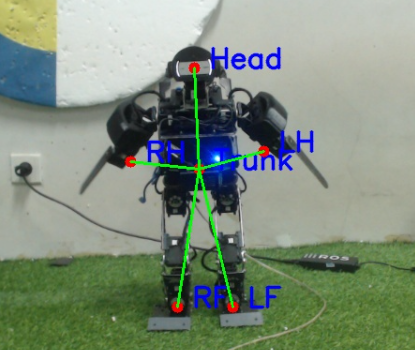
\includegraphics[width=\textwidth]{gambar/robot_6_result.jpg}
      \caption{Robot Image}
      \label{fig:robotimagea}
  \end{subfigure}
     \caption{Comparing Humanoid Robot Pose and Human Pose.}
     \label{fig:comparinga}
\end{figure}

\begin{figure}
  \centering
  \begin{subfigure}[b]{0.45\textwidth}
      \centering
      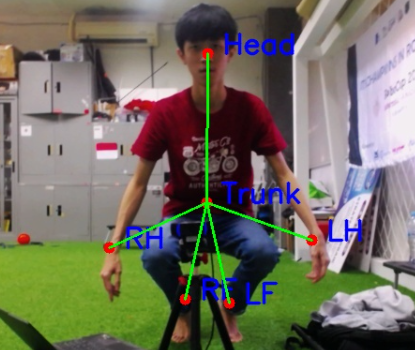
\includegraphics[width=\textwidth]{gambar/human_6_result.jpg}
      \caption{Human Image}
      \label{fig:humanimageb}
  \end{subfigure}
  \hfill
  \begin{subfigure}[b]{0.45\textwidth}
      \centering
      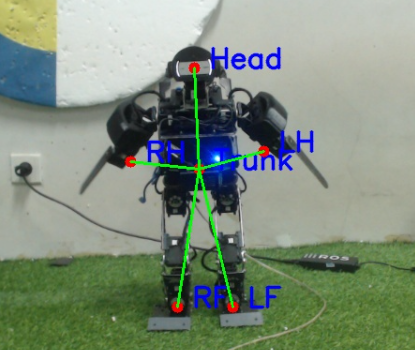
\includegraphics[width=\textwidth]{gambar/robot_6_result.jpg}
      \caption{Robot Image}
      \label{fig:robotimageb}
  \end{subfigure}
     \caption{Comparing Humanoid Robot Pose and Human Pose.}
     \label{fig:comparingb}
\end{figure}

\begin{figure}
  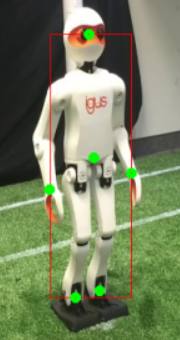
\includegraphics[width=.15\textwidth]{gambar/comp_with_gt/robot_1_gt.png}
  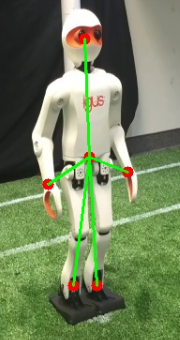
\includegraphics[width=.15\textwidth]{gambar/comp_with_gt/robot_1_res.png} \hfill%
  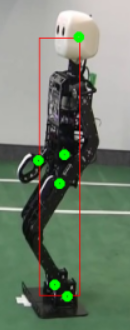
\includegraphics[width=.113\textwidth]{gambar/comp_with_gt/robot_2_gt.png}
  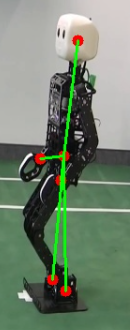
\includegraphics[width=.113\textwidth]{gambar/comp_with_gt/robot_2_res.png} \hfill%
  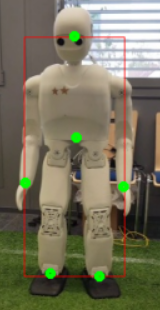
\includegraphics[width=.15\textwidth]{gambar/comp_with_gt/robot_3_gt.png}
  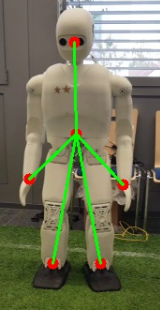
\includegraphics[width=.15\textwidth]{gambar/comp_with_gt/robot_3_res.png}
  \\[\medskipamount]
  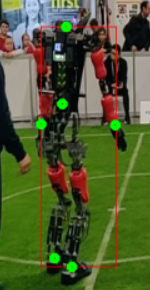
\includegraphics[width=.135\textwidth]{gambar/comp_with_gt/robot_4_gt.png}
  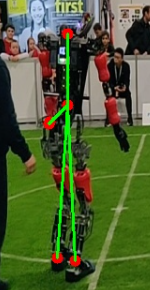
\includegraphics[width=.135\textwidth]{gambar/comp_with_gt/robot_4_res.png} \hfill%
  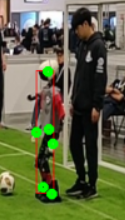
\includegraphics[width=.148\textwidth]{gambar/comp_with_gt/robot_5_gt.png}
  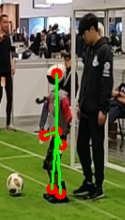
\includegraphics[width=.148\textwidth]{gambar/comp_with_gt/robot_5_res.png} \hfill%
  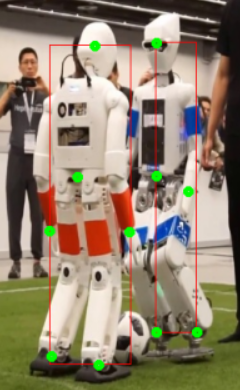
\includegraphics[width=.16\textwidth]{gambar/comp_with_gt/robot_6_gt.png}
  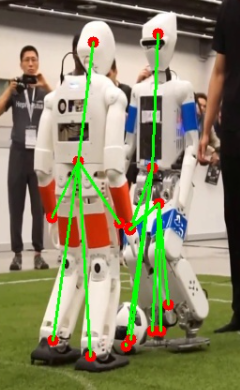
\includegraphics[width=.16\textwidth]{gambar/comp_with_gt/robot_6_res.png}
  \\[\medskipamount]
  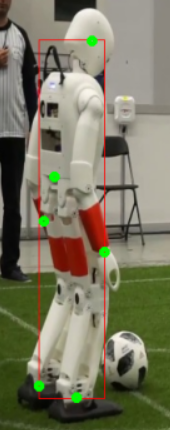
\includegraphics[width=.11\textwidth]{gambar/comp_with_gt/robot_7_gt.png}
  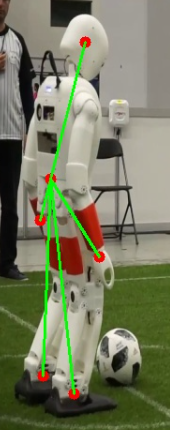
\includegraphics[width=.11\textwidth]{gambar/comp_with_gt/robot_7_res.png} \hfill%
  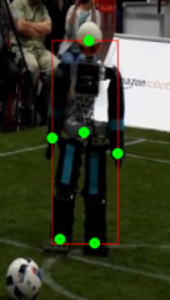
\includegraphics[width=.155\textwidth]{gambar/comp_with_gt/robot_8_gt.png}
  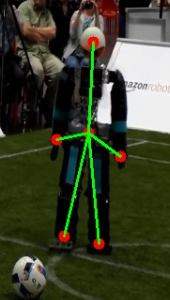
\includegraphics[width=.155\textwidth]{gambar/comp_with_gt/robot_8_res.png} \hfill%
  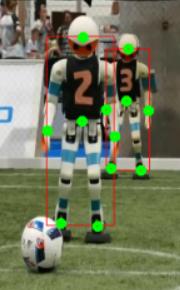
\includegraphics[width=.17\textwidth]{gambar/comp_with_gt/robot_9_gt.png}
  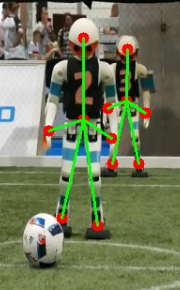
\includegraphics[width=.17\textwidth]{gambar/comp_with_gt/robot_9_res.png}
  \\[\medskipamount]
  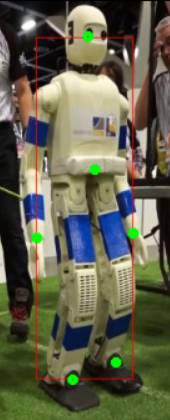
\includegraphics[width=.12\textwidth]{gambar/comp_with_gt/robot_10_gt.png}
  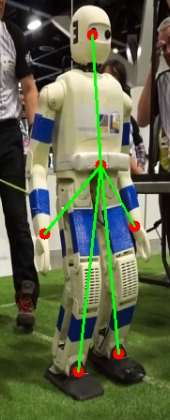
\includegraphics[width=.12\textwidth]{gambar/comp_with_gt/robot_10_res.png} \hfill%
  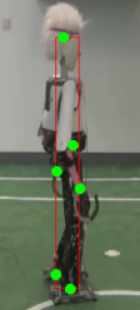
\includegraphics[width=.137\textwidth]{gambar/comp_with_gt/robot_11_gt.png}
  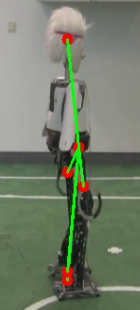
\includegraphics[width=.137\textwidth]{gambar/comp_with_gt/robot_11_res.png} \hfill%
  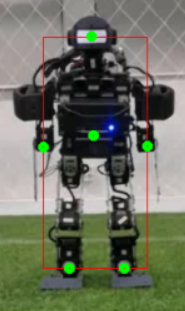
\includegraphics[width=.18\textwidth]{gambar/comp_with_gt/robot_12_gt.png}
  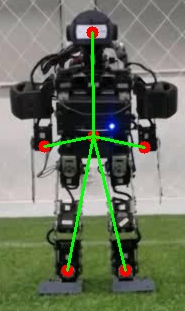
\includegraphics[width=.18\textwidth]{gambar/comp_with_gt/robot_12_res.png}
  \centering
  \captionsetup{justification=centering, margin=2cm}
  \caption{Comparison Between Ground Truth and Detection Result on Every Type of Robot in Dataset}
  \label{fig:comparisongtandresult}
\end{figure}